\documentclass[a4paper,12pt,french] {article}

\usepackage[sujet]{../../../Style}

\fancyhead[L]{02/02/2022}
\fancyhead[C]{\textbf{DS5 : Fonctions polynomiales de degré 2}}
\fancyhead[R]{\premiere ST2S 2}

\renewcommand{\baselinestretch}{1.2}

% Passage en A3
%\geometry{a3paper,landscape,bottom=7mm,twocolumn}
%\setlength{\headwidth}{39cm} %42cm-2*margin pour fancyhdr


\begin{document}

\rem{L'usage de la calculatrice est autorisé. La propreté et l'orthographe seront prises en compte. Tout le devoir peut être fait sur le sujet.}

Nom: \hfill Prénom: \hfill \

\begin{exercice} \

\compo[0.7]
{
On se donne la parabole $\mathscr P$ ci-contre, et $f:x \mapsto ax^2+c$ la fonction de degré deux associée.
\begin{enumerate}
\item Quel est le signe de $a$? \dotfill
\item Donner la valeur de $c$: \dotfill
\item Placer le sommet de $\mathscr P$ et préciser ses coordonnées: \dotfill
\item Quel est l'axe de symétrie de $\mathcal P$? \dotfill
\item Donner les deux racines de $f$: \dotfill
\item En utilisant le point $A(2;-1)$, déterminer $a$, et en déduire l'équation de $\mathscr P$, sous forme développée puis factorisée.
\end{enumerate}
}
{
\begin{centrer}
\begin{tikzpicture}[scale=\echellepgf]
\begin{axis}[
styleglobal,
width=0.9*\echellepgfinv*\linewidth,
xmin=-4, xmax=4,
ymin=-5, ymax=5,
xtick distance=1,
ytick distance=1,
]
\addplot[styleplot,domain=(-4:4)]{(0.5*x^2-3} node[pos=0.6,below right]{$\mathscr P$};;
\end{axis}
\end{tikzpicture}
\end{centrer}
}
\points 5
\end{exercice}

\begin{exercice}
Une entreprise produit mensuellement entre 200 et 3 000 panneaux solaires.\\
On modélise le résultat de l'entreprise réalisé sur la vente de $x$ centaines de panneaux
solaires par la fonction $f$ définie sur l'intervalle $[2~; ~30]$ par : $$f(x)=-2x^2+50x-200$$

\begin{enumerate}
\item On admet que, pour tout $x$ de l'intervalle  $[2~; ~30]$, on a $f(x)=-2(x-20)(x-5)$.\\
Dresser le tableau de signes de la fonction $f$ sur l'intervalle $[2~; ~30]$:
\compo[0.4]
{
\points 6
}
{
\begin{center}
\begin{tikzpicture}
\tkzTabInit[lgt=2.5]{ /1, /4}{2,,30}
\end{tikzpicture}
\end{center}
}
\item A quels volumes de production de panneaux solaires le résultat réalisé par
l'entreprise est-il positif ?

\points 3

\item Déterminer la valeur du bénéfice maximal et le volume de production correspondant.

\points 3

\end{enumerate}
\end{exercice}

\begin{exercice} \

\begin{enumerate}
\item En justifiant, relier chacune des paraboles $\mathscr P_1$, $\mathscr P_2$ et $\mathscr P_3$ aux fonctions ci-dessous:

\compo[0.4]
{
\begin{itemize}[leftmargin=20pt]
\item $f:x \mapsto (x-1)(x+3)$
\item $g:x \mapsto -2x^2+2$
\item $h:x \mapsto 5(x-0.5)(x+0.5)$

\points {10}

\end{itemize}
}
{
\begin{centrer}
\begin{tikzpicture}[scale=\echellepgf]
\begin{axis}[
styleglobal,
width=0.9*\echellepgfinv*\linewidth,
xmin=-4, xmax=4,
ymin=-5, ymax=5,
xtick distance=1,
ytick distance=1,
]
\addplot[styleplot]{((x-1)*(x+3)} node[pos=0.524,above right]{$\mathscr P_1$};
\addplot[styleplot,color=blue,densely dashed]{-2*x^2+2} node[pos=0.6,above right]{$\mathscr P_2$};
\addplot[styleplot,color=red,densely dotted]{5*(x-0.5)*(x+0.5)} node[pos=0.535,above right]{$\mathscr P_3$};
\end{axis}
\end{tikzpicture}
\end{centrer}
}

\item On considère la fonction $i:x \mapsto y=-0.5(x+2)(x-3)$. Tracer la parabole associée à la fonction $i$ sur le repère ce-dessous. Si besoin, on pourra noter des calculs ci-dessous.

\points 4

\begin{centrer}
\begin{tikzpicture}[scale=\echellepgf]
\begin{axis}[
styleglobal,
width=0.9*\echellepgfinv*\linewidth,
xmin=-6, xmax=6,
ymin=-4, ymax=3,
xtick distance=1,
ytick distance=1,
]
%\addplot[styleplot]{0.5*(x+2)*(x-3)};
\end{axis}
\end{tikzpicture}
\end{centrer}

\item Dresser le tableau de variations de $i$. Justifier.

\compohaut[0.5]
{
\points 5
}
{
\begin{center}
\begin{tikzpicture}
\tkzTabInit[lgt=1.2]{ /1, /3}{$- \infty$,,$+ \infty$}
\end{tikzpicture}
\end{center}
}

\end{enumerate}
\end{exercice}

\begin{exercice} \

\compo[0.5]
{\strut
On s'intéresse à la trajectoire d'un ballon de
basketball lancé par un joueur faisant face
au panneau. Cette trajectoire est modélisée
dans le repère ci-contre.

Dans ce repère, l'axe des abscisses
correspond à la droite passant par les pieds
du joueur et la base du panneau.

On suppose que la position initiale du
ballon se trouve au point $J$ et que le segment
$[AB]$ représente le panneau sur lequel il
faut que le ballon rebondisse pour atteindre
le panier.

La trajectoire du ballon est assimilée à la courbe $\mathscr C_f$ représentant une fonction $f$.
}
{
\begin{centrer}
\begin{tikzpicture}[scale=\echellepgf]
\begin{axis}[
styleglobal,
hauteurproptick,
width=0.9*\echellepgfinv*\linewidth,
xmin=-0.5, xmax=6,
ymin=-0.5, ymax=5.5,
xtick distance=1,
ytick distance=1,
ylabel style={sloped like y axis,anchor=north east},
%ylabel style={at={(ticklabel cs:1)},anchor=near ticklabel opposite,rotate=90},
ylabel={Hauteur (m)},
xlabel={Distance (m)},
%xlabel near ticks,
%ylabel near ticks,
%xlabel shift={5mm},
%major grid style={line width=1pt},
]
\addplot[styleplot,domain=(0:4)]{-0.4*x^2+2.2*x+2} node[pos=0.9,above right] {$\mathscr C_f$};
\node[stylepoint,inner sep=1pt,fill=blue,label={-60:A}] (A) at (5.3,2.9) {};
\node[stylepoint,inner sep=1pt,fill=blue,label={60:B}] (B) at (5.3,3.5) {};
\node[stylepoint,inner sep=1pt,fill=blue,label={-60:J}] (J) at (0,2) {};
\draw[very thick] (A) -- (B);
\end{axis}
\end{tikzpicture}
\end{centrer}
}

\begin{enumerate}
\item \textbf{ Étude graphique}:\\
En exploitant la figure, répondre aux questions suivantes:
\begin{enumerate}
\item De quelle hauteur le ballon est-il lancé ?

\points 2

\item Quelle est la hauteur du ballon lorsque $x = 0,5$ m ?

\points 2

\item Quelle semble être la hauteur maximale atteinte par le ballon ?

\points 2

\end{enumerate}
      \item \textbf{Étude de la fonction $f$:}\\
      La fonction $f$ est définie sur l'intervalle $[0; 6]$ par $f(x)= -0,4x^2+2,2x+2$:
      
\begin{enumerate}
\item Calculer $f(2)$ et $f(3,5)$. Interpréter ces résultats par une phrase.

\points 4

\item En utilisant la symétrie de la courbe $C_f$, calculer la hauteur maximale atteinte par le ballon.

\points 4
      
 \end{enumerate}     
\item \textbf{Le joueur a-t-il marqué ?}\\
Le panneau, représenté par le segment $[AB]$, se trouve à une distance de $5,3$ m du joueur.
Le point $A$ est à une hauteur de $2,9$ m et le point $B$ est à une hauteur de $3,5$ m
Le joueur a-t-il marqué ? Justifier par un calcul.

\points 4

\end{enumerate}
\end{exercice}
%\detokenize{%}

\end{document}